\documentclass{article}
\usepackage{tikz}
\usepackage{graphicx}
\usepackage{amsmath}
\usetikzlibrary{shapes.geometric, arrows.meta, positioning}

\tikzstyle{startstop} = [rectangle, rounded corners, minimum width=3cm, minimum height=1cm,text centered, draw=black, fill=gray!20]
\tikzstyle{process} = [rectangle, minimum width=3.5cm, minimum height=1cm, text centered, draw=black, fill=blue!10]
\tikzstyle{decision} = [diamond, minimum width=3.5cm, minimum height=1cm, text centered, draw=black, fill=yellow!20, aspect=2]
\tikzstyle{arrow} = [thick, ->, >=Stealth]

\begin{document}

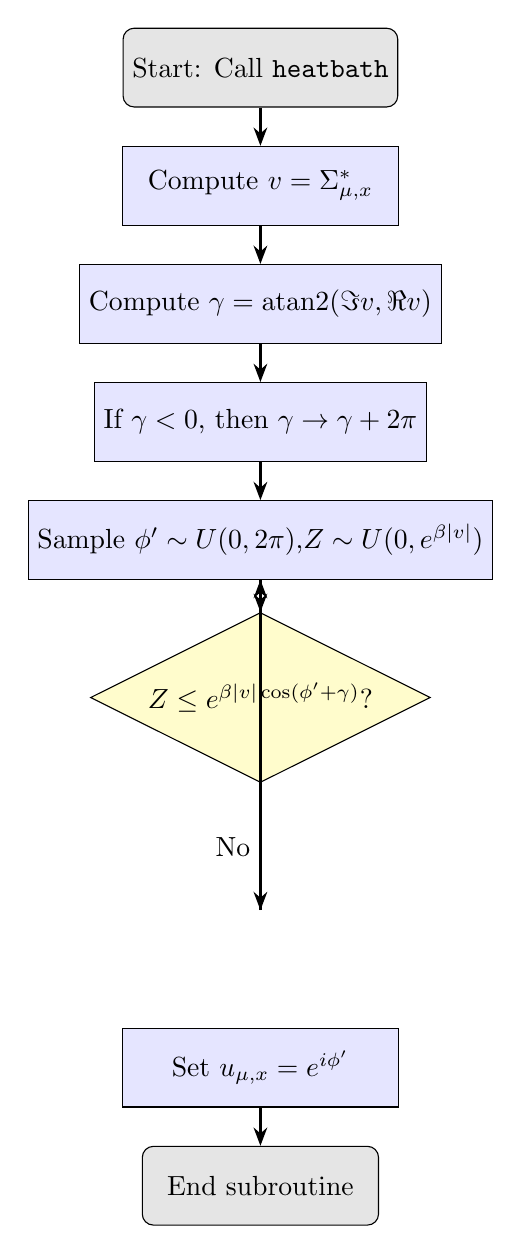
\begin{tikzpicture}[node distance=1.5cm and 2cm]

% Nodes
\node (start) [startstop] {Start: Call \texttt{heatbath}};
\node (staple) [process, below of=start] {Compute $v = \Sigma_{\mu,x}^*$};
\node (params) [process, below of=staple] {Compute $\gamma = \text{atan2}(\Im v, \Re v)$};
\node (gammafix) [process, below of=params] {If $\gamma < 0$, then $\gamma \rightarrow \gamma + 2\pi$};
%\node (initcond) [process, below of=gammafix] {Set \texttt{condition = .false.}};
\node (loopstart) [process, below of=gammafix] {Sample $\phi' \sim U(0,2\pi)$, \\ $Z \sim U(0, e^{\beta|v|})$};
\node (checkZ) [decision, below of=loopstart, yshift=-0.5cm] {$Z \leq e^{\beta|v|\cos(\phi' + \gamma)}$?};
%\node (setcond) [process, right of=checkZ, xshift=5cm] {Set \texttt{condition = .true.}};
\node (repeat) [coordinate, below of=checkZ, yshift=-1.2cm] {};
\node (updateU) [process, below of=repeat, yshift=-0.5cm] {Set $u_{\mu,x} = e^{i\phi'}$};
\node (end) [startstop, below of=updateU] {End subroutine};

% Arrows
\draw [arrow] (start) -- (staple);
\draw [arrow] (staple) -- (params);
\draw [arrow] (params) -- (gammafix);
\draw [arrow] (gammafix) -- (loopstart);
%\draw [arrow] (initcond) -- (loopstart);
\draw [arrow] (loopstart) -- (checkZ);
%\draw [arrow] (checkZ) -- node[above] {Yes} (setcond);
\draw [arrow] (checkZ) -- node[left] {No} (repeat);
%\draw [arrow] (setcond) |- (updateU);
\draw [arrow] (repeat) -- (loopstart);
\draw [arrow] (updateU) -- (end);

\end{tikzpicture}

\end{document}

